\chapter{Conclusions~and~Future~Work}
\label{chap:future} 


\section{Contributions}





\section{Future work}

\subsection{Ensemble training and uncertainty estimation}

There exist a number of uncertainty measures specifically developed for object detection based on Bayesian \gls{NMS} \cite{Harakeh}, test time augmentation {Wei2018} and of particular interest based on ensembles \cite{Le2018}. Some discussion in section--\ref{sec:example_selection}. In future in addition to the simple set of heuristics I would like to make use of ensemble based uncertainty built with k-fold cross-validation. Not only this is beneficial for uncertainty estimation, this form ensemble will make better use of the full dataset not only by improving predictions and providing uncertainty measures, but also by allowing each training image to be also used as a validation image once.

In conflict with our desire to use high resolution images for annotation clarity, ensembles, example selection, and interface responsiveness would all benefit from use of lower resolution images. More experimentation is necessary to determine the best trade off, which seems likely to depend on the dataset.



\subsection{Higher level forms of object detection}

\begin{figure*}[h!]
\begin{subfigure}[t]{1.0\linewidth}
  \centering
  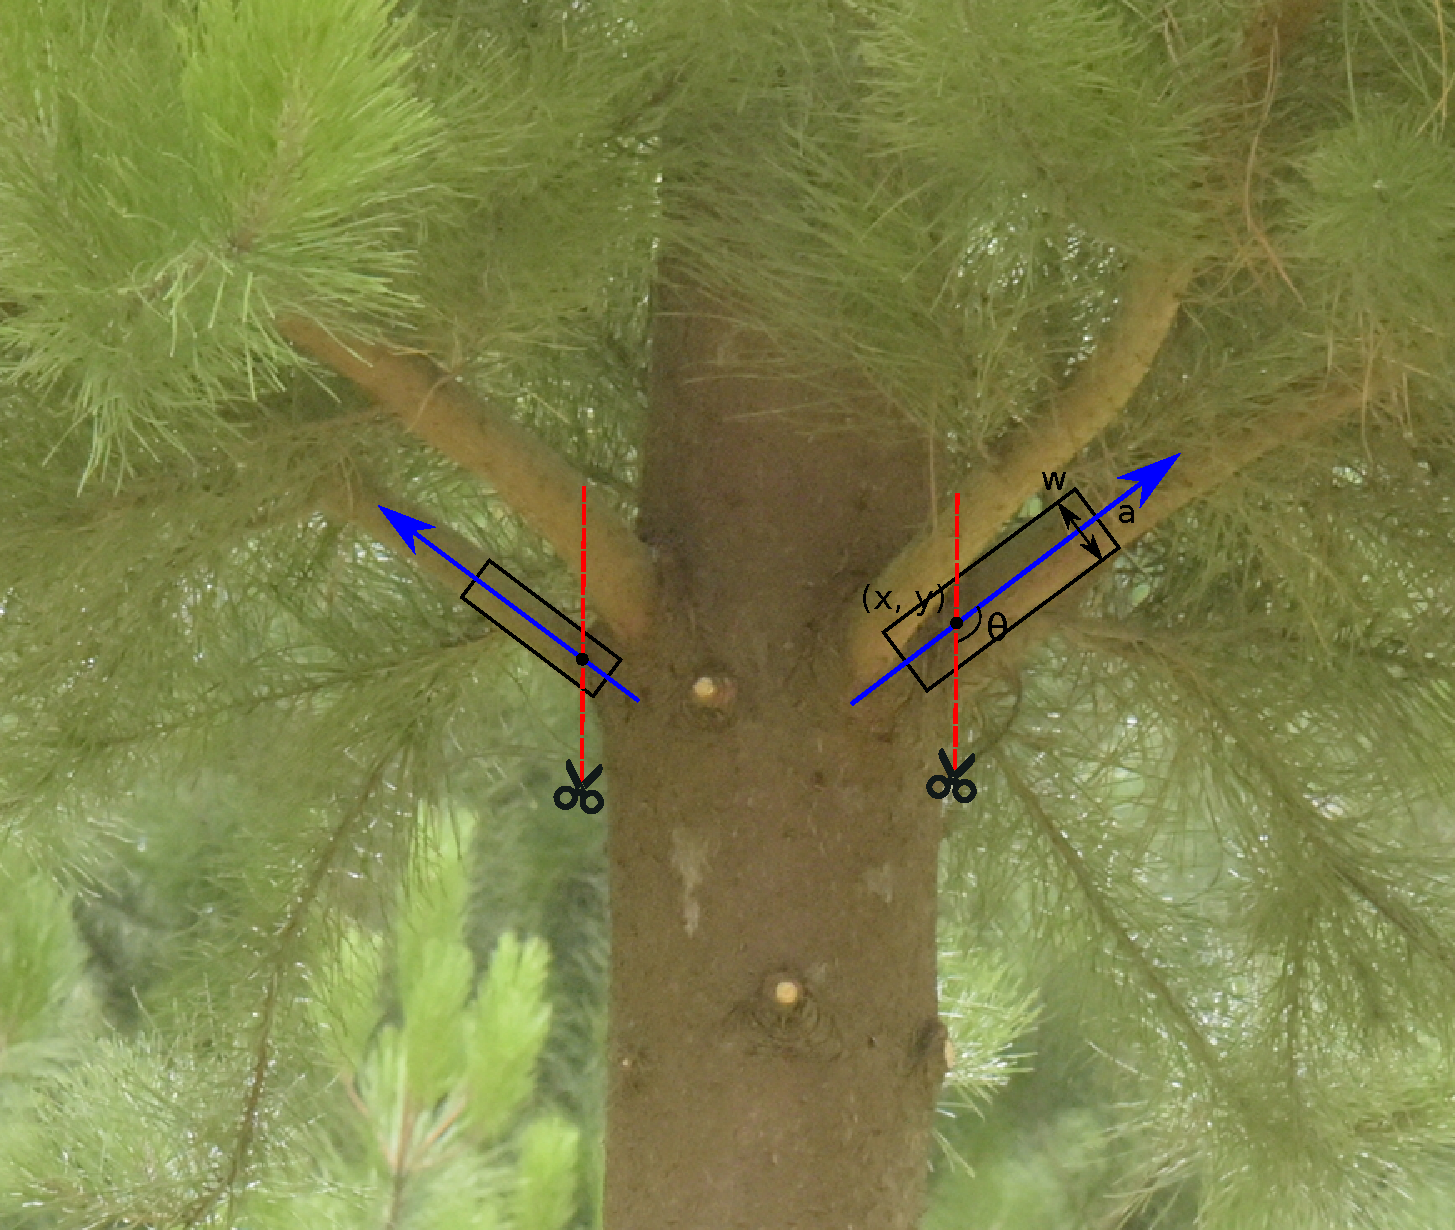
\includegraphics[width=0.8\linewidth]{figures/future/tree_cutpoint.pdf}
  \caption{} 
\end{subfigure}

\begin{subfigure}[t]{1.0\linewidth}
  \centering
  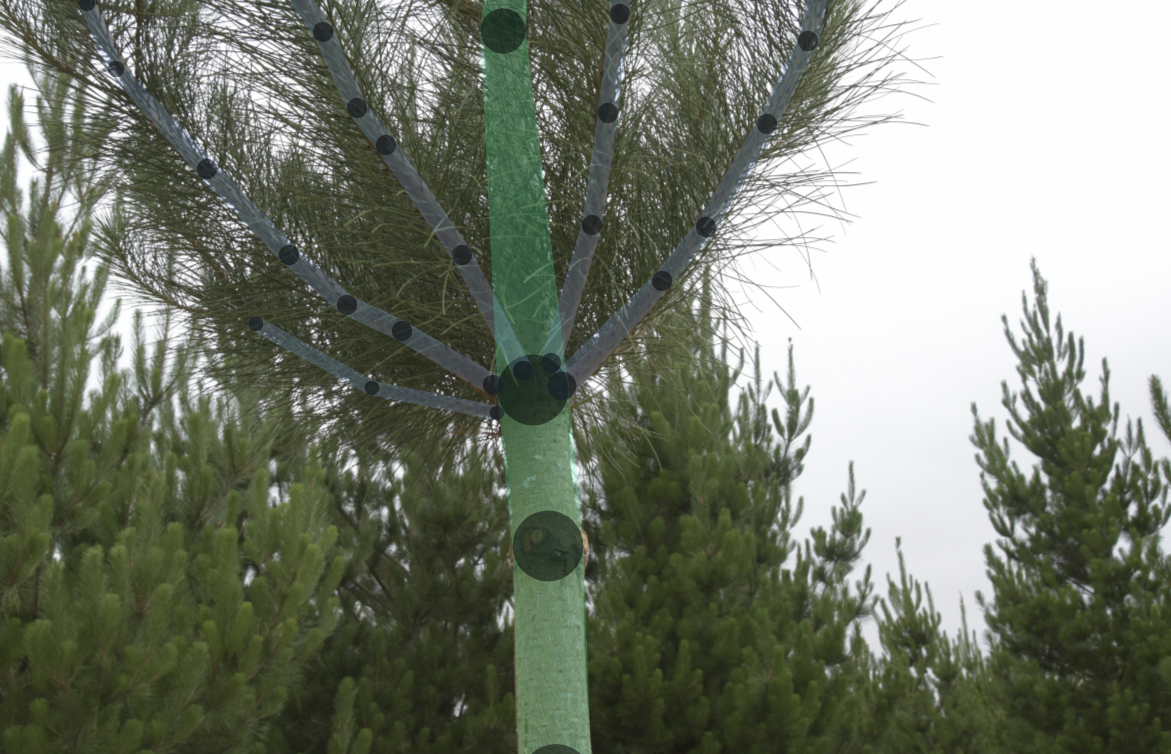
\includegraphics[width=0.8\linewidth]{figures/future/tree_branches.jpg}
  \caption{} 
\end{subfigure}
\caption{Ongoing work into annotating trees in (a) cut-point detection, (b) tree structure skeleton extraction }
\label {fig:future_trees}
\end{figure*}

Bounding boxes have limits for object detection, they only very loosely fit an object. Some objects cannot be described well by bounding boxes at all. Tree branches are fit by bounding boxes very badly; they're very long, and it's not always clear where they start and stop. Figure \ref{fig:future_trees} shows two directions in annotation of tree structures. 

Key-point based detectors are widely used for human pose recognition, I would like to use this form of pose recognition to label other types of object. The branches dataset used as an example in this work is a trial for detecting cut positions, to do this we will modify models which treat objects as key-point detection, for example \cite{Zhou2019} or \cite{Law2018}, both successors to RetinaNet \cite{Wang2017} used in this work. Extracting skeletons are also of interest, where a pose with fixed topology is too limited. Methods used for road network extraction \cite{Li2018}, shape estimation \cite{Jiang2019a} or polygon extraction \cite{Acuna2018} can be modified for example for tree structure extraction. 

One barrier preventing research into new forms of object detection is annotation. Models for detection can be integrated with the verification based annotation approach described in this thesis for experimentation on new domains.

\section{Annotating uncertainty}

In future the ability to annotate images based on uncertainty may be a useful approach, as a means of calibrating confidence and for the purposes of weighting examples in the training process. As opposed to epistemic uncertainty, aleatoric uncertainty can be estimated directly (by a \gls{NN} for example by regression).  

This kind of uncertainty annotation may be also useful in weighting training loss, where the network can place more weight on hard, yet unambiguous examples. The use of Focal Loss means that examples which fail to classify well are weighted much more highly, if these examples are ambiguous because of shadow or lack of resolution - their contribution to the training will be purely as noise.

Hard examples are often cited as being the most useful for an object detector, but if the hard examples are not really hard examples, because they are also visually ambiguous or uncertain (high aleatoric uncertainty) then their usefulness as a learning target might be less, but still possesses value for use in validation and calibration.